% ============================================================
%  CHAPITRE 6 — SPRINT 4 : OPÉRATIONS D'ATELIER ET CYCLE DE VIE
% ============================================================
\chapter{Sprint 4 : Opérations d'Atelier et Cycle de Vie des Interventions}

\chapintro{Ce sprint représente le c\oe ur des opérations de l'atelier~:
affectation des mécaniciens, examens, facturation, approbation client, réparation,
validation et paiement. Toutes ces étapes sont tracées automatiquement par le
\textbf{Intervention Lifecycle Tracker} sur 10 états.}

\section{Introduction}

Une fois le rendez-vous confirmé, le flux opérationnel passe entre les mains de
l'équipe de l'atelier. Un tracker transverse se met à jour automatiquement à chaque
transition, offrant une visibilité totale sur l'état de chaque intervention.

\section{Identification du Backlog Sprint 4}

\begin{table}[H]
\centering
\caption{Backlog Sprint 4 --- Opérations d'Atelier}
\label{tab:backlog-s4}
\begin{tabularx}{\textwidth}{|l|X|l|c|}
\hline
\rowcolor{gray!20}
\textbf{ID} & \textbf{User Story} & \textbf{Priorité} & \textbf{SP} \\
\hline
US15 & Chef~: assigner des mécaniciens à une tâche & \prio{H} & 5 \\[2pt]\hline
US16 & Mécanicien~: consulter ses tâches assignées & \prio{H} & 3 \\[2pt]\hline
US17 & Mécanicien~: soumettre un rapport d'examen & \prio{H} & 5 \\[2pt]\hline
US18 & Chef~: réviser et valider le rapport d'examen & \prio{H} & 3 \\[2pt]\hline
US19 & Chef~: créer et finaliser un devis (facture) & \prio{H} & 5 \\[2pt]\hline
US20 & Client~: approuver ou refuser le devis & \prio{H} & 3 \\[2pt]\hline
US21 & Mécanicien~: soumettre la fin de réparation & \prio{H} & 3 \\[2pt]\hline
US22 & Chef~: valider la réparation et notifier le client & \prio{H} & 3 \\[2pt]\hline
US23 & Admin~: enregistrer le paiement & \prio{H} & 3 \\[2pt]\hline
US24 & Système~: tracer le cycle de vie (10 états) & \prio{H} & 8 \\[2pt]\hline
US25 & Utilisateurs~: notifications in-app et push FCM & \prio{M} & 5 \\[2pt]\hline
US26 & Client~: télécharger la facture en PDF & \prio{M} & 3 \\[2pt]\hline
US27 & Client / Mécanicien~: application Android native & \prio{M} & 13 \\[2pt]\hline
\multicolumn{3}{|r|}{\textbf{Total Sprint 4}} & \textbf{62 SP} \\
\hline
\end{tabularx}
\end{table}

\section{Conception}

\subsection{Diagramme de cas d'utilisation --- Sprint 4}

\begin{figure}[H]
\centering
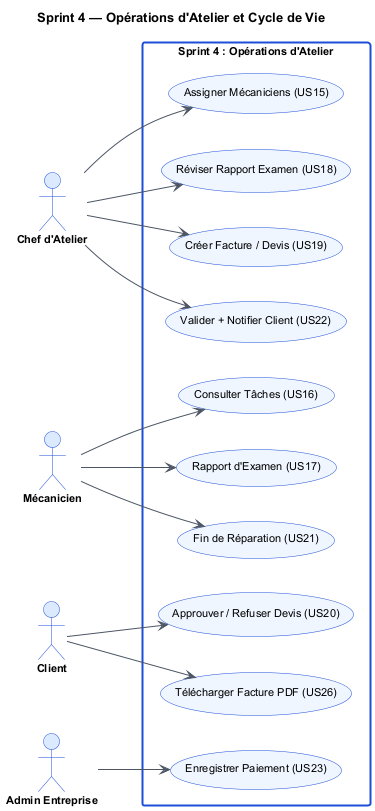
\includegraphics[width=\textwidth,height=0.58\textheight,keepaspectratio]{diagrams/uc_s4.png}
\caption{Diagramme de cas d'utilisation --- Sprint 4}
\label{fig:uc-s4}
\end{figure}

\subsection*{Machine d'états --- Intervention Lifecycle Tracker}

\begin{figure}[H]
\centering
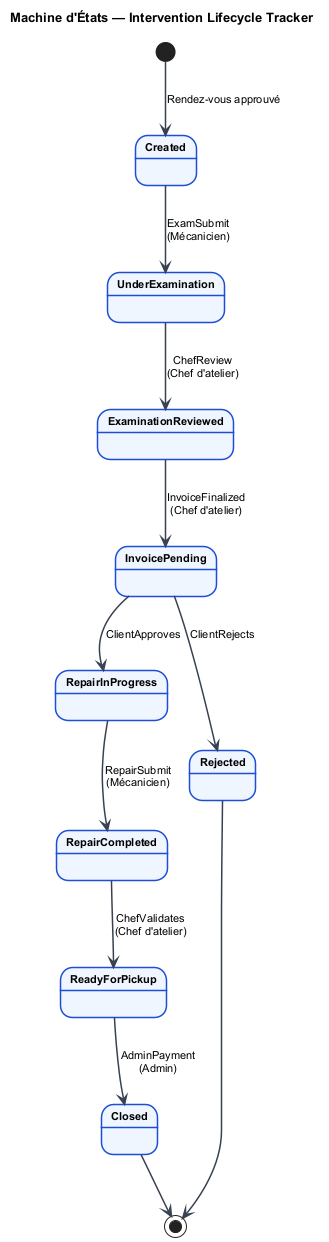
\includegraphics[width=0.72\textwidth]{diagrams/lifecycle.png}
\caption{Machine d'états --- Intervention Lifecycle Tracker}
\label{fig:lifecycle}
\end{figure}

\subsection{Diagramme de classes --- Sprint 4}

\begin{figure}[H]
\centering
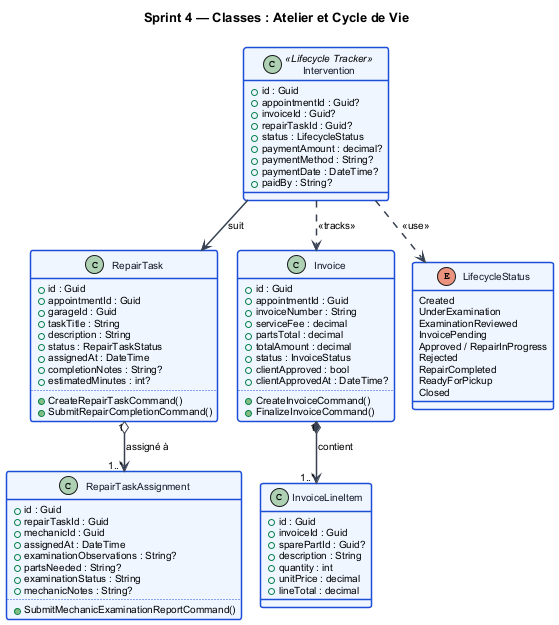
\includegraphics[width=\textwidth,height=0.62\textheight,keepaspectratio]{diagrams/class_s4.png}
\caption{Diagramme de classes --- Sprint 4 (Atelier et Cycle de Vie)}
\label{fig:class-s4}
\end{figure}

\subsection{Diagramme de séquence}

\subsubsection*{SC6 --- Finalisation de Facture et Approbation Client (US19+US20) :
fonctionnalité principale}

\noindent Le chef finalise le devis, le client reçoit une notification et l'approuve.
Le tracker passe à \texttt{InvoicePending} puis \texttt{RepairInProgress}.

\begin{sidewaysfigure}[p]
\centering
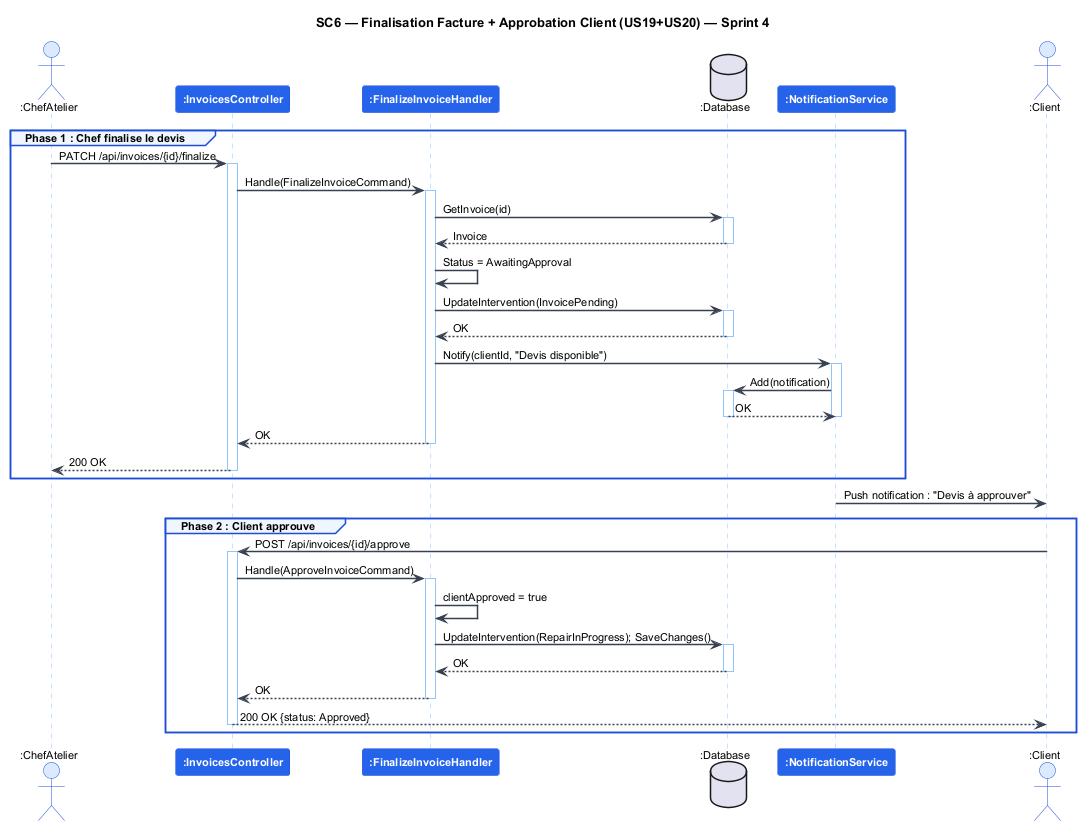
\includegraphics[width=0.92\textheight,keepaspectratio]{diagrams/seq_s4_invoice.png}
\caption{Diagramme de séquence SC6 --- Finalisation et Approbation du Devis}
\label{fig:seq-s4-invoice}
\end{sidewaysfigure}

\section{Conclusion}

Le Sprint 4 a réalisé l'ensemble des opérations métier de l'atelier, de l'affectation
des mécaniciens jusqu'à la clôture de l'intervention. Le \textit{Intervention
Lifecycle Tracker}, mis à jour automatiquement à chaque étape via MediatR, offre
une traçabilité complète. La génération de facture PDF (QuestPDF), les notifications
FCM (Firebase) et l'application mobile Android complètent l'expérience utilisateur.
